\documentclass{article}
\usepackage{graphicx} % Required for inserting images
\usepackage{amssymb, amsmath}
\usepackage{mathtools}
\usepackage{float}
\usepackage{soul}

\title{Solution Fourier Series Triangle Wave}
\author{migue-afk }
\date{February 2023}

\begin{document}

\maketitle

\section{Introduction}
\subsection{General form of Fourier Series}
\begin{equation}
    f(t)=\frac{a_0}{2}+\sum_{n=1}^{\infty} \left [a_n Cos \left ( \frac{2 n \pi}{T}t\right )  + b_n Sin \left ( \frac{2 n \pi}{T}t\right ) \right ]
\end{equation}

\begin{equation}
    a_0=\frac{2}{T} \int_{\frac{-T}{2}}^{\frac{T}{2}}f(t)dt
\end{equation}

\begin{equation}
    a_n=\frac{2}{T} \int_{\frac{-T}{2}}^{\frac{T}{2}}f(t)Cos \left ( \frac{2 n \pi}{T}t\right )dt
\end{equation}

\begin{equation}
    b_n=\frac{2}{T} \int_{\frac{-T}{2}}^{\frac{T}{2}}f(t)Sin \left ( \frac{2 n \pi}{T}t\right )dt
\end{equation}
\subsection{Wave form}


\begin{figure}[h]
    \begin{flushright}
        \centering
       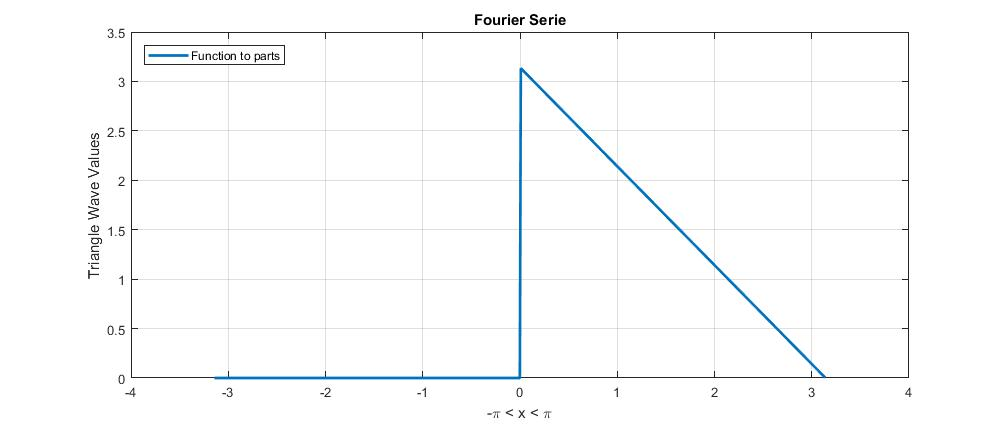
\includegraphics[width=1\textwidth]{n2.jpg}
        \caption{Triangle Wave}
        \label{fig:n2}
    \end{flushright}
\end{figure}

\subsection{Function to parts}
\begin{equation}
    f(t)\begin{Bmatrix}
0 & -\pi< t < 0\\ 
\pi -t & 0 < t <\pi 
\end{Bmatrix}
\quad \text{T= 2$\pi$}
\end{equation}

\subsubsection{Solution}

\begin{equation}
    a_0=\frac{2}{T} \int_{\frac{-T}{2}}^{\frac{T}{2}}f(t)dt = \frac{2}{2 \pi} \int_{\frac{-2 \pi}{2}}^{0}0dt+ \frac{2}{2 \pi} \int_{0}^{\frac{2 \pi}{2}}(\pi - t)dt
\end{equation}

\begin{align*}
    a_0&=\frac{2}{2 \pi} \int_{0}^{\frac{2 \pi}{2}}(\pi - t)dt= \frac{1}{ \pi} \int_{0}^{\pi}(\pi - t)dt\\
    a_0&= \frac{1}{ \pi} \left [\int_{0}^{\pi}\pi dt -  \int_{0}^{\pi}t dt \right ]\\
    a_0&= \frac{1}{ \pi} \left [ \pi t -  \frac{t^2}{2} \right ]_{0}^{\pi}=\frac{1}{ \pi} \left [ \pi (\pi) -  \frac{\pi ^2}{2} \right ]= \frac{1}{ \pi} \left [  \frac{2 \pi^2 -\pi^2}{2} \right ]\\
    a_0&=\frac{1}{ \pi} \left [  \frac{\pi^2}{2} \right ]=\frac{\pi}{2}
\end{align*}

\begin{equation}
\boxed{ a_0=\frac{\pi}{2}}
\end{equation}

\end{document}
